% This file is included in multiple tests (with different drivers)
\documentclass{article}

\usepackage{pgfplots}
\usepgfplotslibrary{external}
\tikzexternalize[force remake]

\usepackage{pgfplots.assert}

\begin{document}
\pgfkeysgetvalue{/tikz/external/system call}\VALUE

\begingroup
\makeatletter
\def\image{image}
\def\texsource{texsource}
\def\EXPECTED{pdflatex \tikzexternalcheckshellescape -halt-on-error -interaction=batchmode -jobname "\image" "\texsource"}%

\def\drivercandidate{pgfsys-pdftex.def}
\ifx\pgfsysdriver\drivercandidate
	\pgfutil@ifundefined{directlua}{%
	}{%
		\def\EXPECTED{lualatex \tikzexternalcheckshellescape -halt-on-error -interaction=batchmode -jobname "\image" "\texsource"}%
	}%
\fi

\def\drivercandidate{pgfsys-xetex.def}
\ifx\pgfsysdriver\drivercandidate
	\def\EXPECTED{xelatex \tikzexternalcheckshellescape -halt-on-error -interaction=batchmode -jobname "\image" "\texsource"}%
\fi

\def\drivercandidate{pgfsys-dvips.def}
\ifx\pgfsysdriver\drivercandidate
	\def\EXPECTED{latex \tikzexternalcheckshellescape -halt-on-error -interaction=batchmode -jobname "\image" "\texsource" %
		&& dvips -o "\image".ps "\image".dvi %
	}%
\fi

\pgfplotsassertequalstok\EXPECTED\VALUE{System call is unexpected}
\endgroup


Bild 1:
\fbox{%
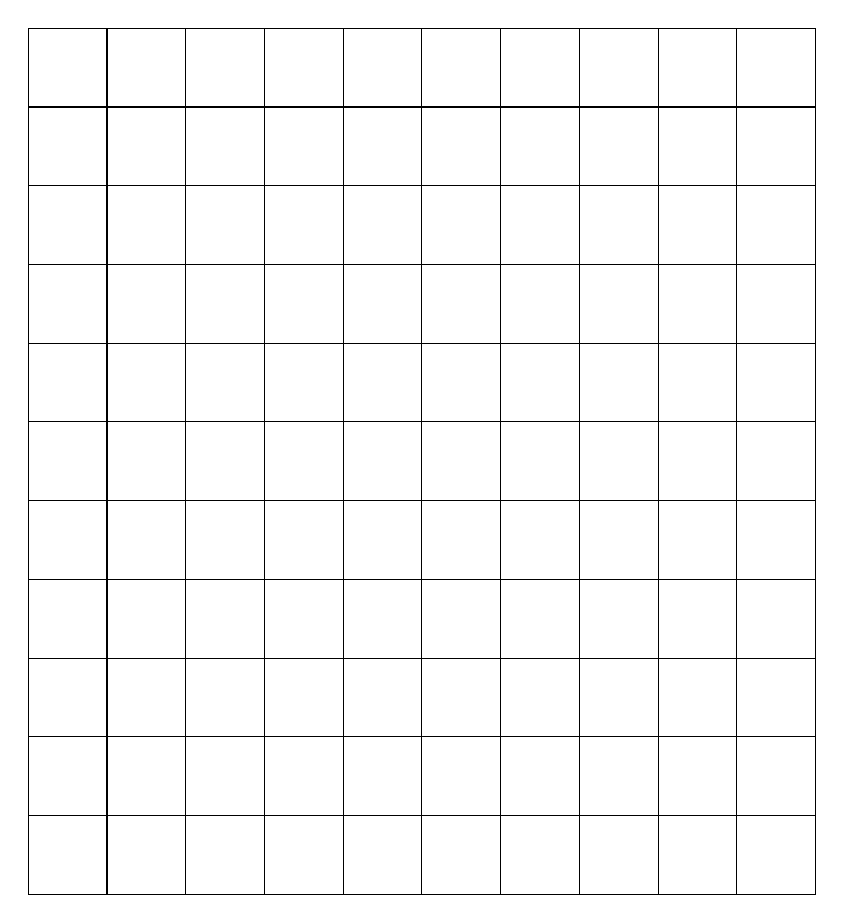
\begin{tikzpicture}
	\draw (0,-1) grid (10,10);
\end{tikzpicture}}

Bild 2:
\fbox{%
Baseline:
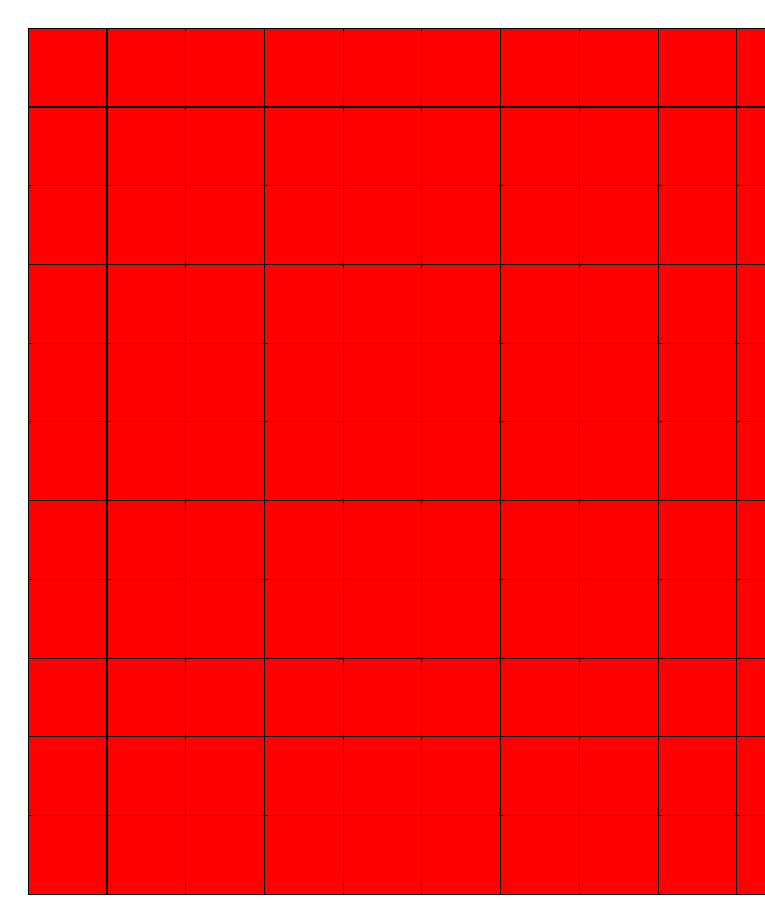
\begin{tikzpicture}[baseline,trim right={(9,0)}]
	\fill[red] (0,-1) rectangle (10,10);
	\draw (0,-1) grid (10,10);
\end{tikzpicture}End Of Trimmed Region
}
\end{document}
